\documentclass{article}

\usepackage{graphicx} % Required for the inclusion of images
\usepackage{natbib} % Required to change bibliography style to APA
\usepackage{amsmath} % Required for some math elements 



\usepackage{amssymb}
\usepackage{amsmath}
\usepackage{float}

\usepackage{caption}

\usepackage{enumitem}
\usepackage{booktabs}

\usepackage{multirow}

\usepackage{amsmath}

\usepackage{subcaption}
\captionsetup{compatibility=false}






\floatstyle{plaintop}
\restylefloat{table}



\setlength\parindent{0pt} % Removes all indentation from paragraphs

\renewcommand{\labelenumi}{\alph{enumi}.} % Make numbering in the enumerate environment by letter rather than number (e.g. section 6)

%\usepackage{times} % Uncomment to use the Times New Roman font

%----------------------------------------------------------------------------------------
%	DOCUMENT INFORMATION
%----------------------------------------------------------------------------------------

\title{Biometrics \\ Laboratory Report} % Title

\author{Jakub \textsc{Ciecierski}} % Author name

\date{\today} % Date for the report

\begin{document}

\maketitle % Insert the title, author and date

\begin{center}
\begin{tabular}{l r}
Date Performed: & October 30, 2015 \\ % Date the experiment was performed
\end{tabular}

\vspace{60pt}

\includegraphics[width=80mm]{res/mini.PNG} \\
\end{center}

% If you wish to include an abstract, uncomment the lines below
% \begin{abstract}
% Abstract text
% \end{abstract}

\newpage

	\tableofcontents
	
\newpage


%----------------------------------------------------------------------------------------

\section{Objective}


%----------------------------------------------------------------------------------------

\section{Convolution Filters} \label{sec:conv}

%----------------------------------------------------------------------------------------
%----------------------------------------------------------------------------------------
\subsection{Introduction}

The main idea of convolution filters is to modify a pixel value based on its neighbourhood.
Value of a given pixel and its neighbours are multiplied by the corresponding element in the \textit{kernel} matrix. We then sum all such products and normalize the final result. This final result is a new value for the given pixel.

Formally

\begin{center}
$I_{out}(x, y) = C_{off} + \frac{\sum_{i} \sum_{j} M(i,j) * I_{in}(x+i, y+j) }{D}$
\end{center}

where:\\
$M$ - is the kernel matrix \\
$I_{in}$ - the input image\\
$I_{out}$ - the output image\\
$C_{off}$ - offset, usually $0$ \\
$D$ - divisor, for filters equal to $\sum_i \sum_j M(i,j)$, for others just $1$\\

Kernel can be of any sizes (e.g. ($3 \times 3$), ($5 \times 5$), ($3 \times 5$), ($15 \times 15$)). The most common ones are probably ($3 \times 3$).

Notice that the summations interval of iterating the kernel matrix has been defined implicitly. To make it easier to compute corresponding pixel we fix a anchor point in the kernel matrix. The anchor point defines the origins of the kernel matrix. The figure~\ref{fig:anchor} shows an example of $3 \times 3$ kernel matrix and matrix of indices of each corresponding element. In this example, the anchor point is fixed in the middle element of kernel matrix, i.e. under value $9$.



\begin{figure}



  \centering

	\begin{tabular}{| r | r | r |}
	\hline
		$-1$ & $-1$ & $-1$ \\
	\hline
		$-1$ & $9$ & $-1$ \\
	\hline
		$-1$ & $-1$ & $-1$ \\
	\hline

	\end{tabular}

	\begin{tabular}{| r | r | r |}
	\hline
		$p_{(-1,-1)}$ & $p_{(-1,0)}$ & $p_{(-1,1)}$ \\
	\hline
		$p_{(0,-1)}$ & $p_{(0,0)}$ & $p_{(0,1)}$ \\
	\hline
		$p_{(1,-1)}$ & $p_{(1,0)}$ & $p_{(1,1)}$ \\
	\hline

	\end{tabular}
  
  {
  \caption{Kernel matrix, and their relative positions}
  \label{fig:anchor}
  }



\end{figure}



It is probably appropriate to mention that convolution filters require quite a lot of computational power. Given a kernel matrix of size $n \times m$, calculation of a single pixel require $m*n$ multiplications. Thus for big kernel matrices the computations might become very slow.

%----------------------------------------------------------------------------------------
%----------------------------------------------------------------------------------------
\subsection{Example}

The example in figure~\ref{fig:convo} will hopefully make it clear how exactly convolution filters define value for a given pixel. The left most matrix presents an input image, the middle one is a kernel and the right most is a final result of the current pixel. The current pixel is marked with red border. The green border however, defines the neighbourhood of that pixel. It should be clear that the anchor point is again fixed under the middle point of the kernel matrix, thus defining its origins. Further, each pixel of the image matrix is multiplied by corresponding kernel value. All products are summed. Since the only pixel that is not multiplied by $0$ has $42$, the final result is simply $42$.


\begin{figure}[H]
\centering

  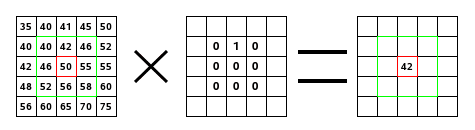
\includegraphics[width=0.9\linewidth]{res/convo.png}
  
\caption{Example of convolution filter. The computation of a new value for pixel in red border. On the left: image matrix. On the right: kernel matrix. The right side is a new value for the current pixel}
\label{fig:convo}
\end{figure}

%----------------------------------------------------------------------------------------
%----------------------------------------------------------------------------------------
\subsection{Special Cases}


Finally special cases that might occur during computation of convolution filters are discussed. Firstly, however obvious, it is important that the final result is clipped to appropriate range. In case of standard RBG $[0 ,255]$, we must ensure that the final values are within this range. Finally, what happens when we compute pixels that lay at the edge of the image. For instance, for the first pixel (starting from upper left corner), the corresponding pixel of kernel matrix will simply not exist. One of the following three solutions can be applied to fix that issue.
\begin{enumerate}
	\item Compute as if there was additional row or column of pixel with values equal to the pixels at the edge.
	\item Skip the pixels with neighbours outside the edge of an image.
	\item The pixels in the neighbourhood outside the edge of an image assume to have value 0.
	\item Wrap the image. pixel outside left edge use values of pixel on the right edge.
\end{enumerate}

%----------------------------------------------------------------------------------------
%----------------------------------------------------------------------------------------
\subsection{Implementation}

The general algorithm flow of convolution filter is presented:
 
\begin{enumerate}
	\item For $input$ image, make a $output$ copy.
	\item For each pixel in the input image.
	\begin{enumerate}	
		\item Compute new value using kernel matrix. The neighbourhood is also taken from input image.
		\item Save new value to output image.
	\end{enumerate}
\end{enumerate}


First of all, the implementation of the main function called $compute$ is shown in figure~\ref{fig:alg_compute}. The $compute$ method calls $computeKernelColor$ for each pixel. The implementation of this method is presented in figure~\ref{alg_compute_kernel}. The details of $computeKernelColor$ method are now discussed. First of all, the two loops represent the summation over the kernel matrix. The $sRange$ and $eRange$, standing for start range and end range respectively, corresponds to the indices of kernel matrix relative to the anchor point. The $getKernelPoint$ is a simply method which returns the value of kernel value for indices relative to the anchor point. This method is shown in figure~\ref{fig:alg_getKernelPoint}. Notice that $kernelMatrix$ is one-dimensional vector.



\begin{figure}[H]
\centering

  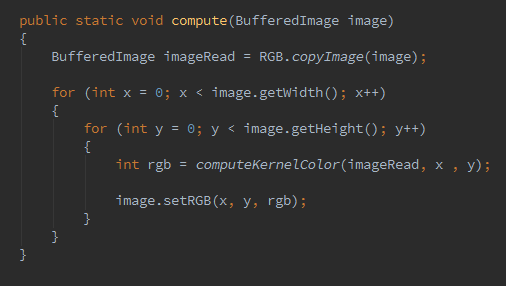
\includegraphics[width=0.9\linewidth]{res/algorithms/compute.png}
  
\caption{Main function of convolution filter}
\label{fig:alg_compute}
\end{figure}






\begin{figure}[H]
\centering

  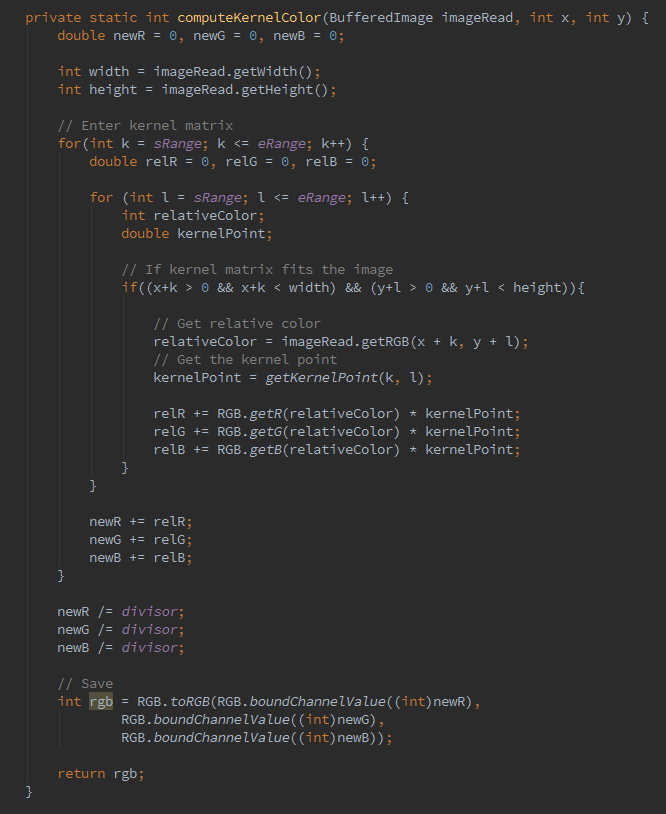
\includegraphics[width=0.9\linewidth]{res/algorithms/computeKernel.png}
  
\caption{Compute Kernel}
\label{fig:alg_compute_kernel}
\end{figure}





\begin{figure}[H]
\centering

  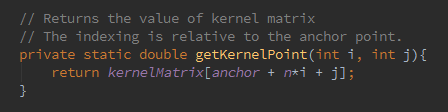
\includegraphics[width=0.9\linewidth]{res/algorithms/getKernelPoint.png}
  
\caption{Get Kernel Point}
\label{fig:alg_getKernelPoint}
\end{figure}


%----------------------------------------------------------------------------------------
%----------------------------------------------------------------------------------------
\subsection{High Pass Filter}

High pass filters underscore components of the image with high frequency. Main objective of these filters is to sharpen an image. In other words, high pass filters preserve the high frequency information and reduce low frequency information.

\begin{figure}[H]
\centering

  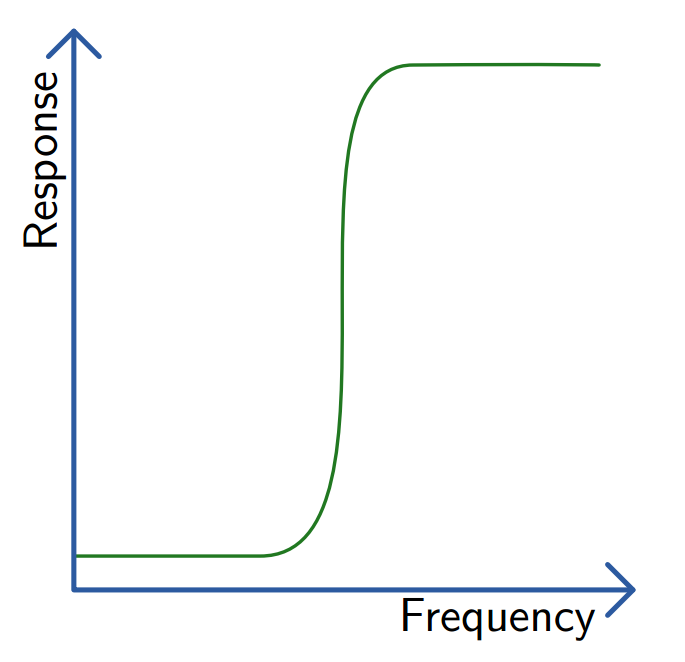
\includegraphics[width=0.5\linewidth]{res/high_pass_graph.png}
  
\caption{High Pass Filter}
\label{fig:high_pass_graph}
\end{figure}


The implementation of an example of an high pass filter called a sharpen filter is shown in figure~\ref{fig:alg_high_pass}.  The kernel is a $3 \times 3$ matrix with anchor point in the middle of that matrix. It was mentioned before that the kernel matrix is implemented using one dimensional vector. Thus it is clear to see that $kernelMatrix[anchor] = 9$

\begin{figure}[H]
\centering

  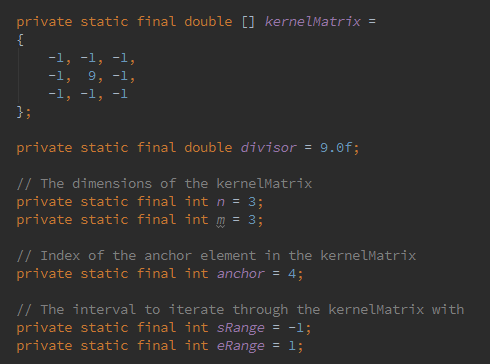
\includegraphics[width=0.9\linewidth]{res/algorithms/high_pass.png}
  
\caption{High Pass Filter}
\label{fig:alg_high_pass}
\end{figure}


%----------------------------------------------------------------------------------------
%----------------------------------------------------------------------------------------
\subsection{Low Pass Filter}

Low pass filter are used to smooth an image. By analogy, the low pass filters, preserve low frequency information and reduce the high frequency information.
Implementation presented in figure~\ref{fig:alg_low_pass}.

\begin{figure}[H]
\centering

  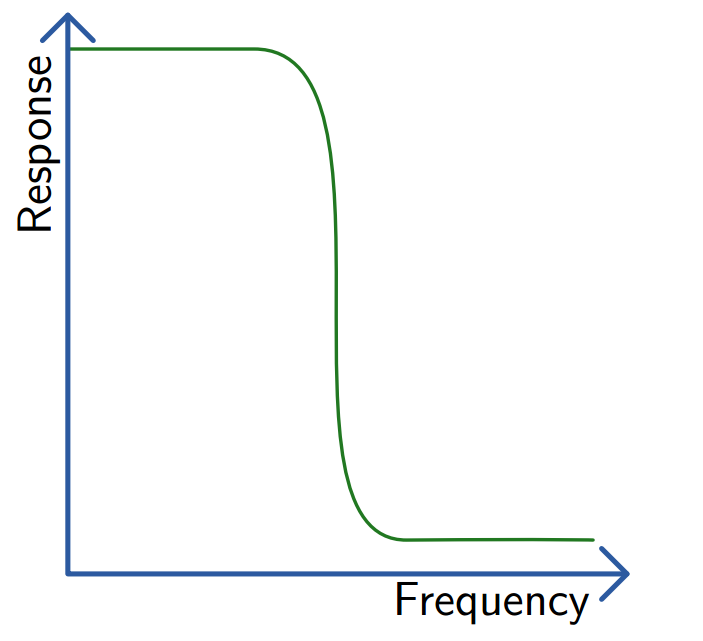
\includegraphics[width=0.5\linewidth]{res/low_pass_graph.png}
  
\caption{Low Pass Filter}
\label{fig:low_pass_graph}
\end{figure}


\begin{figure}[H]
\centering

  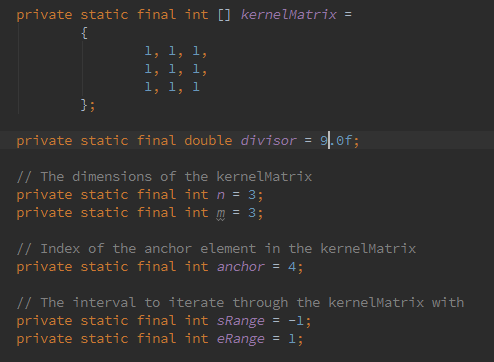
\includegraphics[width=0.9\linewidth]{res/algorithms/low_pass.png}
  
\caption{Low Pass Filter}
\label{fig:alg_low_pass}
\end{figure}

%----------------------------------------------------------------------------------------
%----------------------------------------------------------------------------------------
\subsection{Gaussian Filter}
Gaussian filter is a low pass filter which is used to blur an image.

Figure~\ref{fig:alg_gauss} shows implementation.

\begin{figure}[H]
\centering

  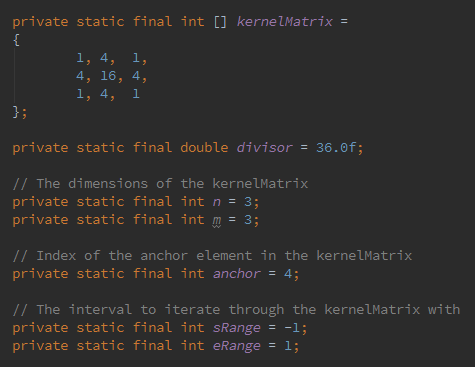
\includegraphics[width=0.9\linewidth]{res/algorithms/gaussian.png}
  
\caption{Gaussian Filter}
\label{fig:alg_gauss}
\end{figure}

%----------------------------------------------------------------------------------------
%----------------------------------------------------------------------------------------
\subsection{Sobel Filter}

In case of Sobel filter, the implementation of $computeKernelColor$ changes



\begin{figure}[H]
\centering

  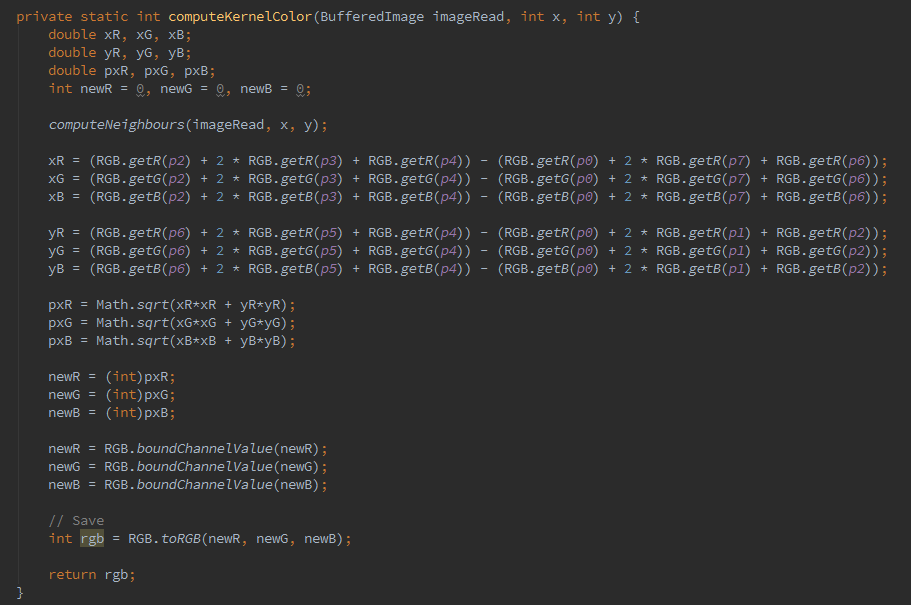
\includegraphics[width=0.9\linewidth]{res/algorithms/computeKernel_sobel.png}
  
\caption{Compute Kernel}
\label{fig:compute_kernel_sobel}
\end{figure}


\begin{figure}[H]
\centering

  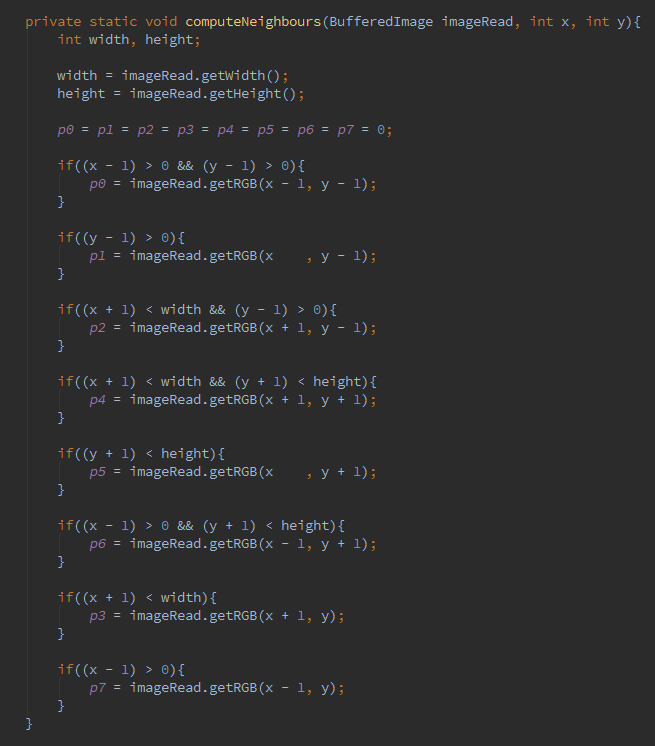
\includegraphics[width=0.9\linewidth]{res/algorithms/computeNeighbours.png}
  
\caption{Compute Kernel}
\label{fig:compute_neigh_sobel}
\end{figure}


%----------------------------------------------------------------------------------------
\section{Pupil}
\label{sec:pupil}

To find the pupil on a image we must first remove as much noise as possible. To achieve this, blur filters are applied. Then, the image should be transformed to binary image - black and white. Further, Sobel filter will ensure that only edges of the pupil are left. At this point, the image should contain only one closed region - the pupil. Thus we need to apply an algorithm that finds a closed regions in an image. Once we have atleast one interior point we can apply scan line fill algorithm for that region. The longest line will represent diameter, and middle of that line will be the center of the eye.

Formally the flow of the algorithm for original color image is as follows:

\begin{enumerate}
	\item Blur the original image - loose all the noise.
	\item Convert to Grayscale
	\item Convert Grayscale to Black and White image - binary image
	\item Apply Sobel filter.
	\item Find a closed region in the image - representing the pupil.
	\item Use scan line fill algorithm to find diameter and centre - the longest line will be the diameter.
\end{enumerate}



%----------------------------------------------------------------------------------------
\section{Results}
\label{sec:results}

%----------------------------------------------------------------------------------------
%----------------------------------------------------------------------------------------
\subsection{Filters}
\label{sec:results_filters}



%----------------------------------------------------------------------------------------
%----------------------------------------------------------------------------------------
%----------------------------------------------------------------------------------------
\subsubsection{High Pass}




\begin{figure}[H]
\centering

\begin{subfigure}{.5\textwidth}
  \centering
  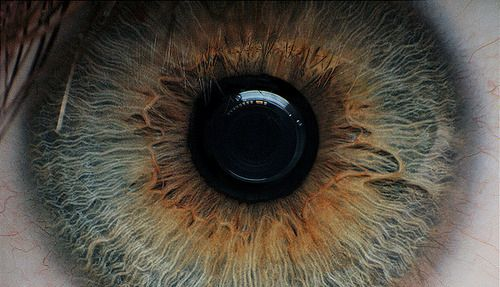
\includegraphics[width=0.9\linewidth]{res/index.jpg}
  \caption{Original image}
  \label{fig:original_img}
\end{subfigure}%
\begin{subfigure}{.5\textwidth}
  \centering
  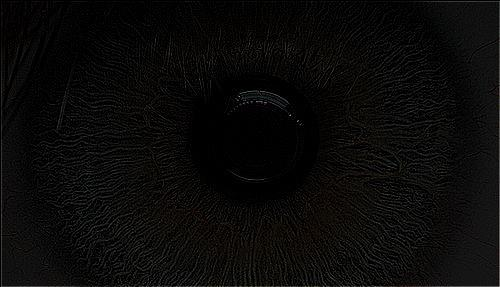
\includegraphics[width=0.9\linewidth]{res/high_pass.jpg}
  \caption{High Pass filter}
  \label{fig:gray_img}
\end{subfigure}

\caption{The original and High Pass filter}
\label{fig:result_high}
\end{figure}






%----------------------------------------------------------------------------------------
%----------------------------------------------------------------------------------------
%----------------------------------------------------------------------------------------
\subsubsection{Low Pass}




\begin{figure}[H]
\centering

\begin{subfigure}{.5\textwidth}
  \centering
  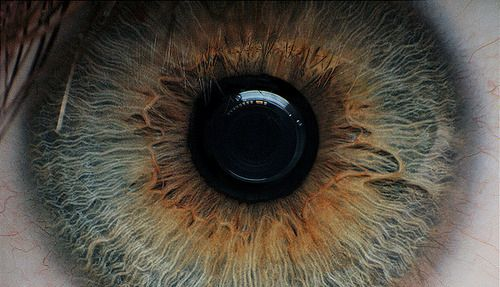
\includegraphics[width=0.9\linewidth]{res/index.jpg}
  \caption{Original image}
  \label{fig:original_img}
\end{subfigure}%
\begin{subfigure}{.5\textwidth}
  \centering
  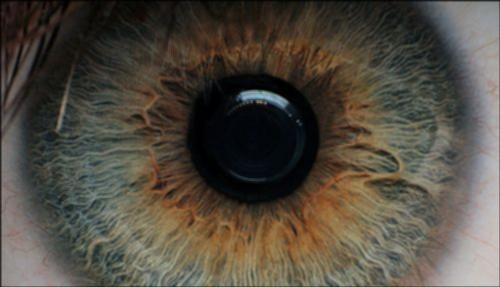
\includegraphics[width=0.9\linewidth]{res/low_pass.jpg}
  \caption{Low Pass}
  \label{fig:gray_img}
\end{subfigure}

\caption{The original and Low Pass filter}
\label{fig:source_img}
\end{figure}


%----------------------------------------------------------------------------------------
%----------------------------------------------------------------------------------------
%----------------------------------------------------------------------------------------
\subsubsection{Gaussian}



\begin{figure}[H]
\centering

\begin{subfigure}{.5\textwidth}
  \centering
  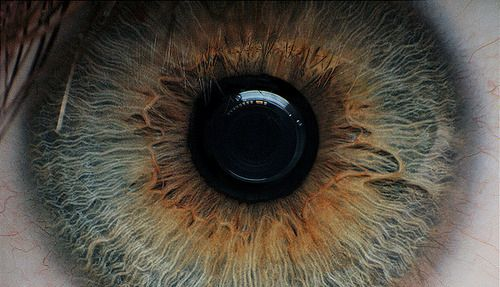
\includegraphics[width=0.9\linewidth]{res/index.jpg}
  \caption{Original image}
  \label{fig:original_img}
\end{subfigure}%
\begin{subfigure}{.5\textwidth}
  \centering
  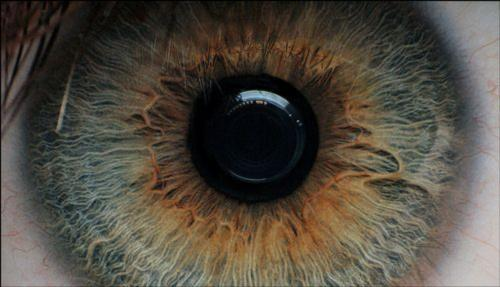
\includegraphics[width=0.9\linewidth]{res/gaussian.jpg}
  \caption{Gaussian Filter}
  \label{fig:gray_img}
\end{subfigure}

\caption{The original and gaussian filter}
\label{fig:result_gauss}
\end{figure}




%----------------------------------------------------------------------------------------
%----------------------------------------------------------------------------------------
%----------------------------------------------------------------------------------------
\subsubsection{Sobel}


\begin{figure}[H]
\centering

\begin{subfigure}{.5\textwidth}
  \centering
  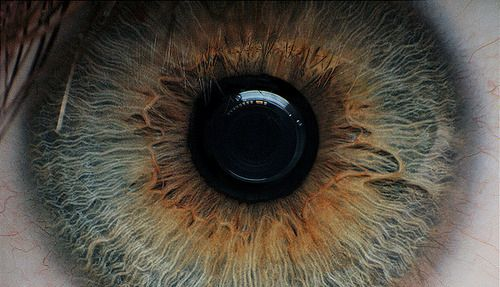
\includegraphics[width=0.9\linewidth]{res/index.jpg}
  \caption{Original image}
  \label{fig:original_img}
\end{subfigure}%
\begin{subfigure}{.5\textwidth}
  \centering
  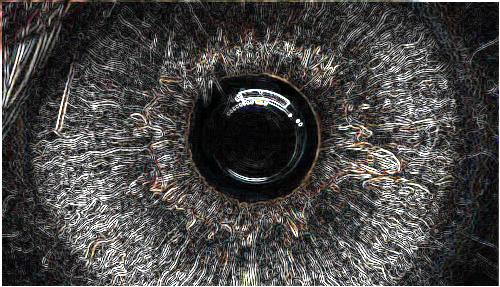
\includegraphics[width=0.9\linewidth]{res/sobel.jpg}
  \caption{Sobel filter}
  \label{fig:gray_img}
\end{subfigure}

\caption{The original and Sobel filter}
\label{fig:source_img}
\end{figure}


%----------------------------------------------------------------------------------------
%----------------------------------------------------------------------------------------
\subsection{Pupil}
\label{sec:results_pupil}

The results of finding the pupil is now presented. First, the original image is subjected to low pass filtering. In this test case, the low pass filter was applied twice. Blurring is shown in figure~\ref{fig:result_pup_orig_low}. Further, figure~\ref{fig:result_pup_low_gray} transforms the image to grayscale. By trail and error a threshold value 10 has been chosen to thresholding presented in figure~\ref{fig:result_pup_gray_tresh}. Finally, the last filter applied is the Sobel filter in figure~\ref{fig:result_pup_thresh_sobel}.


%%%
%
% Original to Low Pass
%
%%%
\begin{figure}[H]
\centering

\begin{subfigure}{.3\textwidth}
  \centering
  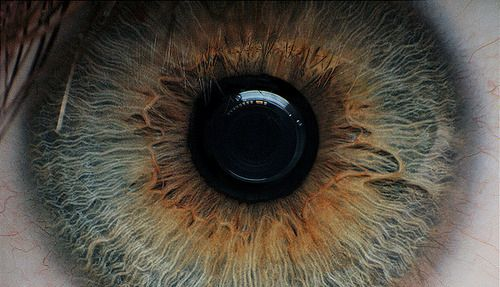
\includegraphics[width=0.9\linewidth]{res/index.jpg}
  \caption{Original image}
  \label{fig:}
\end{subfigure}%
\begin{subfigure}{.3\textwidth}
  \centering
  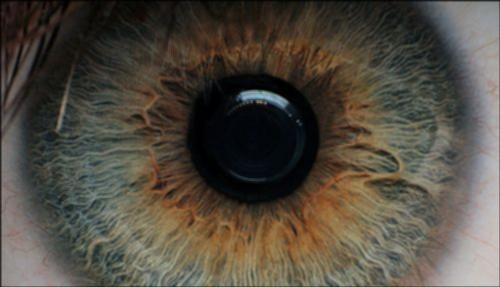
\includegraphics[width=0.9\linewidth]{res/pupil/low_pass_n.jpg}
  \caption{Low Pass filter}
  \label{fig:}
\end{subfigure}
\begin{subfigure}{.3\textwidth}
  \centering
  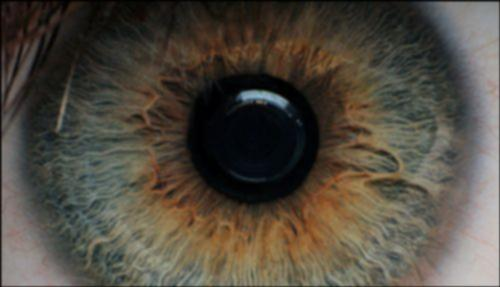
\includegraphics[width=0.9\linewidth]{res/pupil/low_pass_nn.jpg}
  \caption{Double Low Pass filter}
  \label{fig:}
\end{subfigure}


\caption{Original to Double Low Pass filter}
\label{fig:result_pup_orig_low}
\end{figure}


%%%
%
% Low Pass to Grayscale
%
%%%
\begin{figure}[H]
\centering

\begin{subfigure}{.5\textwidth}
  \centering
  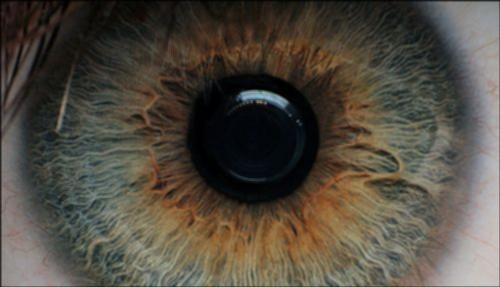
\includegraphics[width=0.9\linewidth]{res/pupil/low_pass_n.jpg}
  \caption{Original image}
  \label{fig:original_img}
\end{subfigure}%
\begin{subfigure}{.5\textwidth}
  \centering
  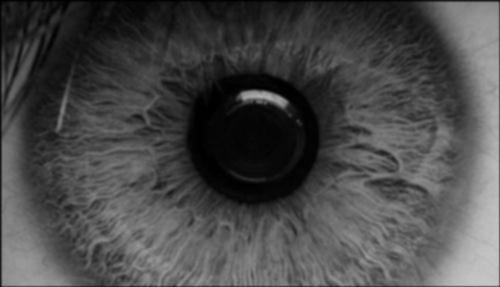
\includegraphics[width=0.9\linewidth]{res/pupil/gray_n.jpg}
  \caption{Grayscale image}
  \label{fig:gray_img}
\end{subfigure}


\caption{Low Pass to Grayscale}
\label{fig:result_pup_low_gray}
\end{figure}





%%%
%
% Grayscale to Threshold
%
%%%
\begin{figure}[H]
\centering

\begin{subfigure}{.5\textwidth}
  \centering
  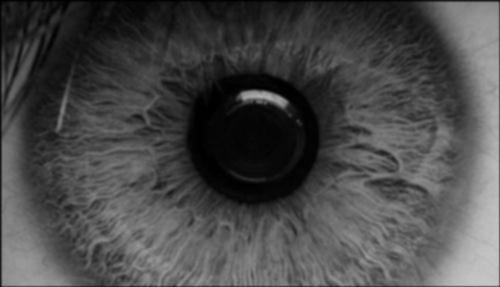
\includegraphics[width=0.9\linewidth]{res/pupil/gray_n.jpg}
  \caption{Original image}
  \label{fig:original_img}
\end{subfigure}%
\begin{subfigure}{.5\textwidth}
  \centering
  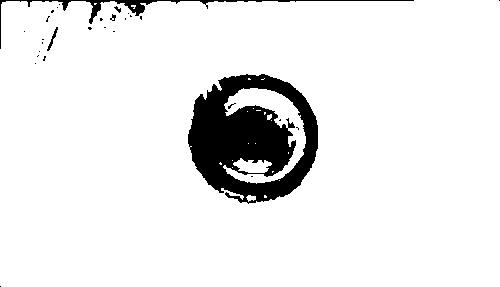
\includegraphics[width=0.9\linewidth]{res/pupil/thresh_n10.jpg}
  \caption{Thresholding with threshold equal to 10}
  \label{fig:gray_img}
\end{subfigure}


\caption{Grayscale to Threshold 10}
\label{fig:result_pup_gray_tresh}
\end{figure}




%%%
%
% Threshold to Sobel
%
%%%
\begin{figure}[H]
\centering

\begin{subfigure}{.5\textwidth}
  \centering
  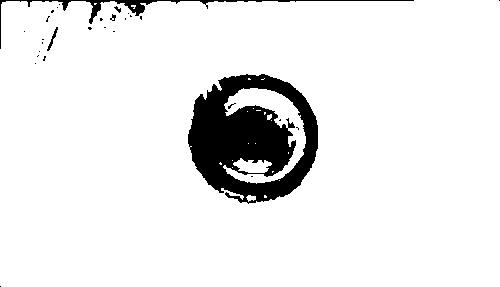
\includegraphics[width=0.9\linewidth]{res/pupil/thresh_n10.jpg}
  \caption{Original image}
  \label{fig:original_img}
\end{subfigure}%
\begin{subfigure}{.5\textwidth}
  \centering
  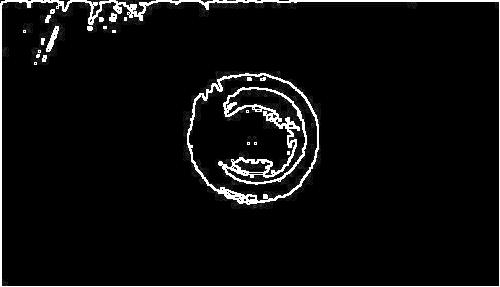
\includegraphics[width=0.9\linewidth]{res/pupil/sobel_n.jpg}
  \caption{Sobel filter}
  \label{fig:gray_img}
\end{subfigure}


\caption{Binary to Sobel filter}
\label{fig:result_pup_thresh_sobel}
\end{figure}





%----------------------------------------------------------------------------------------
%	BIBLIOGRAPHY
%----------------------------------------------------------------------------------------

\bibliographystyle{apalike}

\bibliography{sample}
%http://docs.gimp.org/en/plug-in-convmatrix.html

%----------------------------------------------------------------------------------------


\end{document}